\section{Method}

\subsection{Task Formulation}

\hspace{1pc}We use imitation learning (IL) to train the proposed BID.
In IL, expert first demonstrates a driving action $a_{t}$ (such as steering, brake and throttle) in response to an input frame $f_t$ based on the expert's policy $\pi(f_{t})$.
It reflects the expert's driving skills, judgement, and behavior.
The core idea of IL is to train the proposed BID agent to replicate the expert's actions by learning from these observed interactions.


Before training the BID using IL, we first collect a series of frame and action pairs $(f_{t}, a_{t})$ produced by expert demonstrations.
These data is then utilized to train the BID policy $\pi_{\theta}(f_{t})$, which approximated the expert's policy.
%The overall objective of imitation is 
%\begin{equation} \label{eq:target}
%	\argmin_{\theta} \mathbb{E}_{(\mathbf{f}_{i}, \mathbf{a}_{i})\sim \mathcal{D}} \left[ \mathcal{L}(\pi_{\theta}(\mathbf{f}_{i}), \mathbf{a}_{i}) \right] \enspace .
%\end{equation}
%
In the validating phase, we on longer utilize the expert's strategy, but only the trained BID policy.

\begin{figure*}[t]
	\centering
	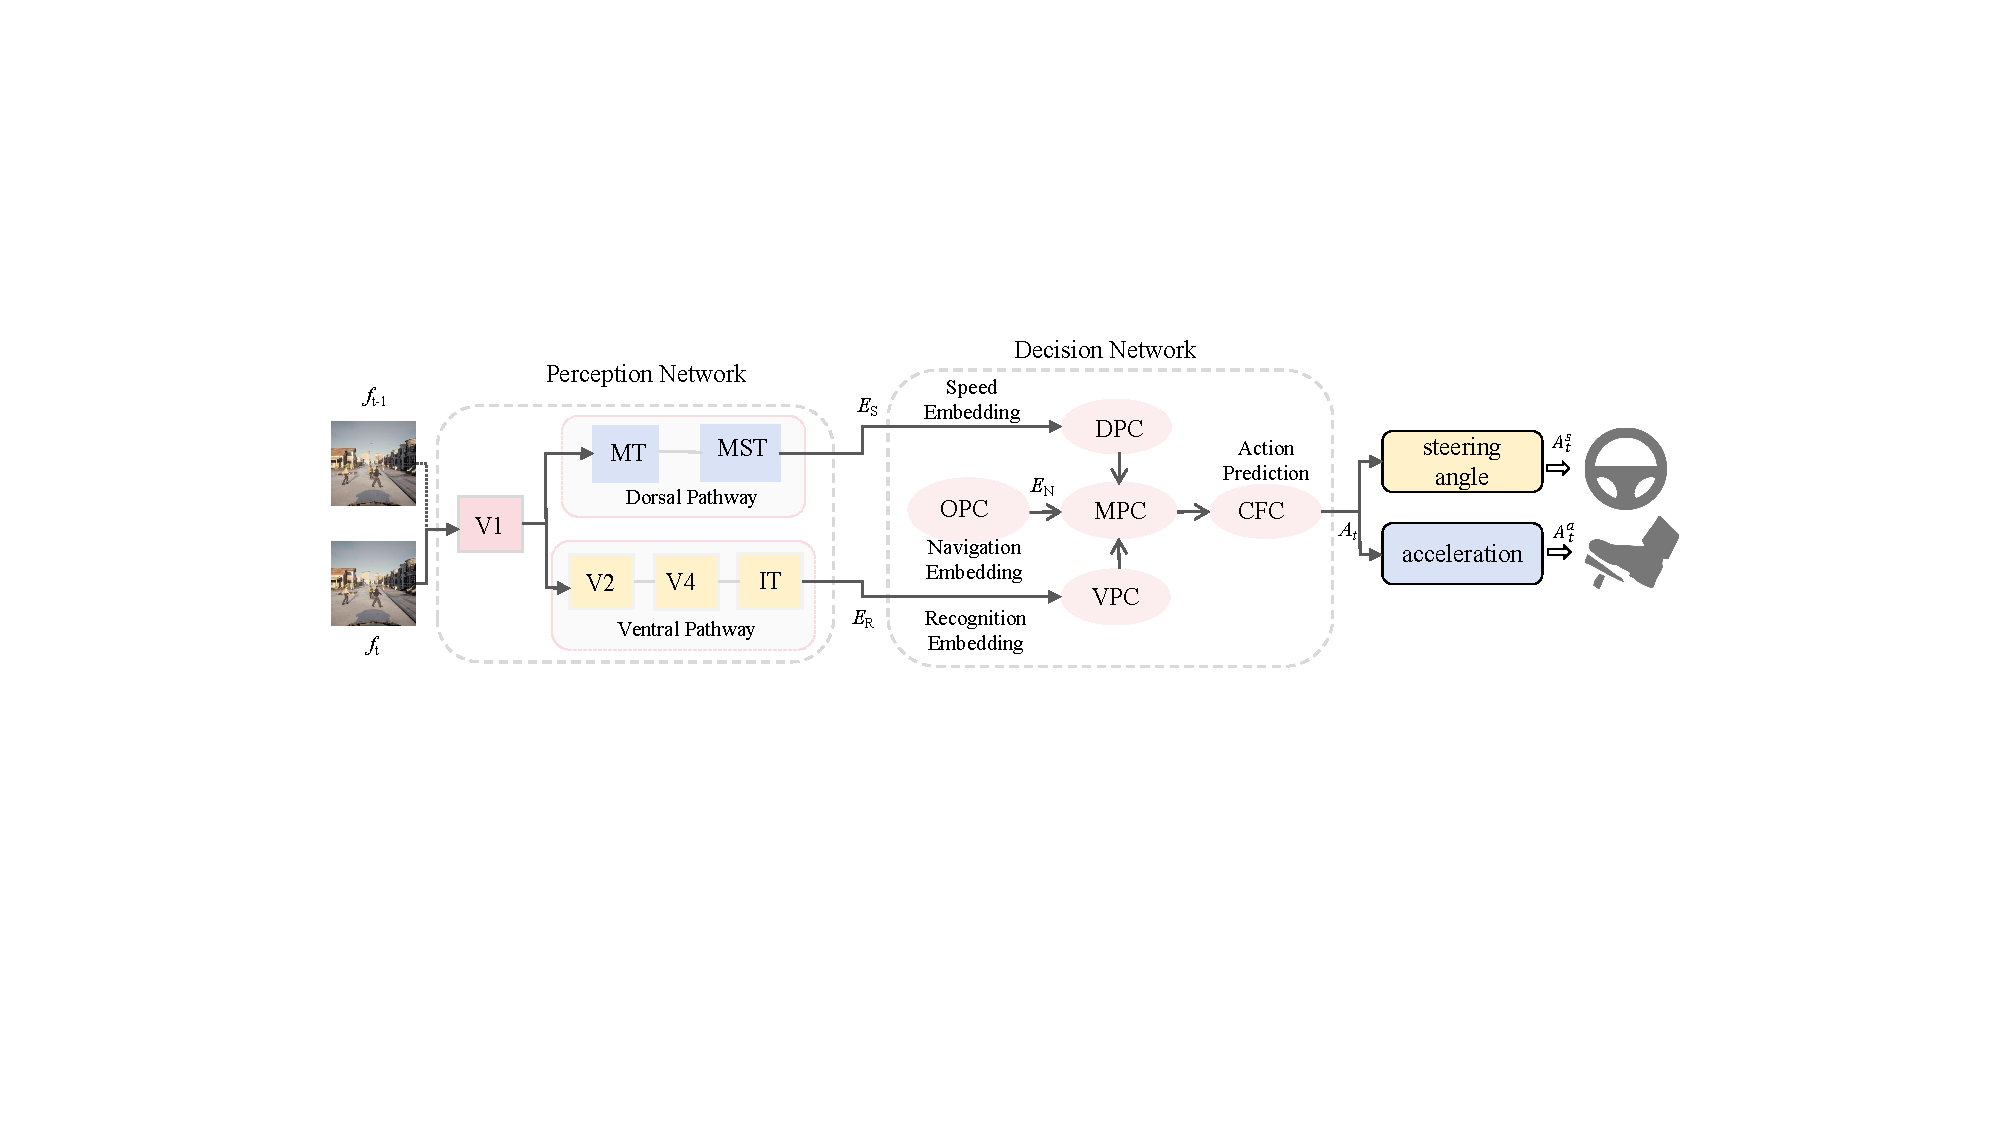
\includegraphics[width=\linewidth]{fig/net.pdf}
	\caption{The network architecture of the BID agent is primarily composed of two main components: the perception network and the decision network.
	The perception network includes both the dorsal and ventral pathways, which allow the system to understand and process its surroundings.
	The decision network consists of five modules that represent different regions of the prefrontal cortex: the medial prefrontal cortex (VPC), orbital prefrontal cortex (OPC), caudal prefrontal cortex (CPC), dorsal prefrontal cortex (DPC), and ventral prefrontal cortex (VPC). 
	Specifically, the input to the system is an RGB image $ \mathbf{F}_{t} $, which represents the current visual scene.
	The output is the action $\mathbf{a}_{i}$, which directly controls the ego-vehicle's maneuvering.
	The action $A_\text{t}$ includes the steering angle $ A_t^s $ and acceleration $ A_t^a $ of the vehicle, making BID a pure vision-based, end-to-end autonomous driving model.
	It is important to note that these action components are automatically associated with the captured images during the data collection process.
	}
	\label{fig:fig2}
\end{figure*}


\subsection{Neural Aligned BID}
\hspace{1pc}Inspired by the brain's remarkable capabilities in perception and decision-making, we have proposed the perception and decision network based on neural pathway anatomical alignment to simulate the information processing mechanisms of brain into an autonomous driving system. 
This approach is designed to significantly improve both the interpretability and robustness of the system.

\subsubsection{Perception Network}
\hspace{1pc}As shown in Fig.~\ref{fig:fig2}, our brain-inspired perception network begins by capturing precise input data from the surrounding environment, which includes essential traffic elements such as roads, vehicles, pedestrians, and traffic signals. 
% 模型的输入
% the ego vehicle's forward speed $s_t\in\mathbb{R}$
% data $f_t$ consists of 3 horizontally continuous frames from camera.
% s $f_{t}=\{f_{t,1}, f_{t,2}, f_{t,3} \}$
At time $t$, the input frame $f_t$ is processed through a series of deep convolutional neural networks and recurrent networks, incorporating activation functions commonly used in deep neural networks. 
This processing mirrors the way external information is handled by the brain's visual cortex. 
Initially, the primary visual cortex (V1) processes the visual input, extracting key features. 
To manage the high computational demands, the first area, V1$_\text{BID}$, performs a 7$\times$7 convolution with stride 2, followed by 3$\times$3 max pooling with stride 2, and another 3$\times$3 convolution. 
These features are then passed along to the dorsal visual pathway, where areas such as middle temporal (MT) and middle superior temporal (MST) specialize in encoding motion and velocity information between current frame $ f_t $ and previous frame $ f_{t-1} $, particularly related to spatial location and movement\cite{wang2022btn}. 
The dorsal pathway is implemented as a dynamic filter network\cite{jia2016dynamic} and utilized to extract the spatial relation between background and foreground, 
and use appearance repsentation $ \alpha_t $ to dynamically infer convolutional filter.


% 腹侧
At the same time, the ventral pathway receives these features, with inferior temporal (IT) cortex focusing on encoding object category information, thereby facilitating object recognition.
% Cornet
Each visual area in ventral pathway implements a specific neural circuitry, where neurons perform simple, canonical computations, such as convolution, addition, nonlinearity, response normalization, and pooling over a receptive field. 
The structure of the circuitry is identical across all visual areas, though the total number of neurons in each area may vary.
The subsequent areas, V2$_\text{BID}$, V4$_\text{BID}$ and IT$_\text{BID}$, each carry out two 1$\times$1 convolutions, a bottleneck-style 3 $ \times $ 3 convolution with stride 2 (which expands the number of features by a factor of four), and another 1$\times$1 convolution. 
To simulate recurrence, the outputs of each area are fed back into the same area 4 times for further processing.


%
After this sequence of processing steps, our network is capable of efficiently extracting and outputting multi-dimensional embeddings of the current environment to next decision network. 
These features include both the appearance characteristics $ E_\text{S} $ of objects and motion-related information $ E_\text{S} $.



\subsubsection{Decision Network}
% 决策模块
The output features from the perception network are then efficiently passed to a brain-inspired decision-making network, where they undergo further processing through transformer networks, along with anatomical alignment to the prefrontal cortex pathway. 
This simulates how sensory information is processed by different regions of the prefrontal cortex in the brain.
%


% 腹侧
The ventral prefrontal cortex (VPC) generates goals based on recognition embedding (visual cues), allowing for quick responses and adaptation to changes in the environment.
%
In our setup, we flatten the embedding patches and then fed it into the transformer model.
To provide positional context for each token, we apply a standard learnable 1D positional embedding $\mathbf{p}\in \mathbb{R}^{S\times c}$~\cite{Alexey:2021}, and add this embedding directly to the token.


% 背侧
The dorsal prefrontal cortex (DPC) is responsible for generating goals based on sequences, as well as temporal and spatial environmental cues, offering clear guidance for decision-making and action.
% 眶额
Within this process, the orbitofrontal cortex (OFC) plays a crucial role in establishing future action goals $n_t$, which is encoded as a one-hot command embedding.
It helps to clarify and focus on the desired objectives. 
% 速度、导航命令
The navigation command $n_t$ is mapped into a vector embedding $E_\text{N}$ using a fully connected layer.
% and forward speed $s_t$



% 内侧
The medial prefrontal cortex (MPC) is critical for making decisions based on current states, along with a high-level navigation command.
It ensure that our actions are optimized according to previous experiences and future goal.
The input embeddings of MPC are merged with the output of VPC, DPC and OPC.
Formally, we define the state encoder for the current state $O_t=(f_t, n_t)$, parameterized by $ \pi_{\theta}(f_t, n_t) $, as
\begin{equation}\label{eq:encoder}
	A_\text{t}^\text{s}, A_\text{t}^\text{s} = \pi_\text{MPC}(E_\text{s}, E_\text{N}, E_\text{V}).
%	e_{\theta}: \mathbb{R}^{|\mathbf{X}_{t}|\times W\times H\times3}\times\mathbb{R}\times \mathbb{R}^k \rightarrow \mathbb{R}^{S \times c} \enspace .
\end{equation}


Navigation embedding $E_{t}$ is used as a switch to activate various MLP branches for inferring $A_{t}$ in CIL \cite{Codevilla:2018} and CILRS \cite{Codevilla:2019}. 
However, in our approach, we treat $E_{t}$ as an input signal to be processed by a transformer. 
We found no significant differences between these two methods, and treating $n_{t}$ as an input signal simplifies the training process.
%
% 注意力学习
% 连接3个图像
To effectively associate multi-view information, we leverage the attention mechanism of transformers\cite{Vaswani:2017}. 
This approach allows the model to learn the relationships between distant image patches (tokens), enabling it to associate feature map patches across different views ({\ie}, from horizontal 3 perspectives of the ego-vehicle). 


% CFC
In the MPC embedded space, we learn a scenario embedding using a transformer encoder composed of $L$ multi-head attention layers. 
Each layer includes multi-headed self-attention~\cite{Vaswani:2017}, layer normalization~\cite{Ba:2016}, and feed-forward MLP modules. 
% 尾侧
The caudal prefrontal cortex (CPC) is crucial for searching, identifying, and locating specific targets, ensuring that we can accurately focus on and navigate towards these targets. 
The final output is obtained by linearly projecting the concatenated outputs of each attention head, which are then passed to the action prediction module.
We use $L=4$ layers, each with $4$ attention heads. 
The hidden dimension $D$ of the transformer layer is set to match the output dimension of the ResNet, {\ie}, $D=512$. 
%
% 动作预测
The output from the transformer encoder, with a size of $S\times c$, is average-pooled and passed through an MLP.
This MLP consists of three fully connected layers (FC), with ReLU nonlinearity applied between each layer.
The final output action $A_t\in\mathbb{R}^2$ represents the steering angle and acceleration (brake/throttle), {\ie}, $\mathbf{a}_{t} = (A_{\text{t}^\text{t}}, A_{\text{t}^\text{a}})$. 


% 总结
These regions work together in the decision-making process, forming a highly integrated latent feature vector that effectively captures the essential information needed for making decisions. 
This latent vector is then processed through a carefully constructed hidden layer, which generates accurate and reliable outputs, such as driving actions, value function estimates, and speed control commands.


\subsection{Loss Function}

\hspace{1pc}The BID network is designed to replicate the advanced information processing abilities of the human brain by carefully aligning brain pathways with corresponding network modules. 
Through iterative updates, the network adjusts its parameters to better match human decision-making processes, ultimately improving its performance and accuracy.
%
% 损失函数
At time $t$, given a predicted action $\mathbf{a}_{t}$ and the expert's action(ground truth action) $\hat{\mathbf{a}}_{t}$, we define the training loss as:
\begin{equation}\label{eq:loss}
	\mathcal{L}(\mathbf{a}_t, \hat{\mathbf{a}}_t) = \lambda_{\text{acc}}\lVert a_{\text{acc},t}-\hat{a}_{\text{acc,t}}\rVert_{1} + \lambda_{\text{s}} \lVert a_{\text{s},t}-\hat{a}_{\text{s},t} \rVert_{1} \enspace ,
\end{equation}
where $\lVert\cdot\rVert_{1}$ denotes the $L_1$ distance, $\lambda_{acc}$ and $\lambda_s$ represent the weights assigned to the acceleration and steering angle loss, respectively.
In our setup, both steering angle and acceleration are constrained within the range of $[-1, 1]$, with negative values indicating braking and positive values corresponding to throttle.
The weights are set as $\lambda_{acc} = \lambda_{s} = 0.5$. 


In CILRS \cite{Codevilla:2019}, speed prediction regularization is incorporated into the training loss to address the inertia issue caused by the high likelihood of the ego vehicle remaining stationary in the training data.
However, we did not encounter this problem in our approach, and therefore, the speed prediction branch is not included in our model.
Our results demonstrate that a simple $L_1$ loss is sufficient to achieve strong performance, even in unfamiliar environments.
%
Additionally, the outputs from both the brain-inspired perception network and the brain-inspired decision network are concatenated to form a latent feature that captures critical driving-related information. 
This latent feature is then passed through a hidden layer to map it to driving actions, which also incorporates a feature loss.


%\subsubsection{Brain-Expert Mimetic Entity}
%
%\hspace{1pc}\textbf{\textsf{Agent.}} The BID agent utilizes imitation learning to predict driving behavior based on the current state, supervised by extensive data generated by the reinforcement learning expert. The structure of the agent is illustrated in Fig. \ref{fig:fig2}.

%\textbf{\textsf{Loss Function.}} 
%In the decision-making stage, for each command, a branch is constructed. 
%All branches share the same architecture, with each branch containing an action head for predicting the continuous action $\mathbf{a}$ and a velocity head for predicting the current vehicle speed $\mathbf{s}$. 
%And $\mathbf{\hat{a}}$ represents the expert's action,$\mathbf{\hat{s}}$ is the measured speed, and $\mathbf{a}$ and $\mathbf{s}$ are the actions and speeds predicted by the agent, respectively. 
%\begin{align}
%   \mathcal{L} = \|\hat{\mathbf{a}}-\mathbf{a}\|_{1}^{2} + \lambda_{\mathrm{S}} \cdot (\hat{s}-s)^{2} + \lambda_{\mathrm{F}} \cdot \left\| \mathbf{j}_{\mathrm{NR}}-\mathbf{j}_{\mathrm{BID}} \right\|_{2}^{2}
%\end{align}


\begin{comment}
\subsection{Similarity Metrics}
\hspace{1pc}\textbf{\textsf{Collecting Brain Activation Signals.}} To align the network, we collect the brain's responses to multi-channel grayscale images. Initially, EEG sensors are placed at appropriate locations and connected to data acquisition equipment. Subsequently, neuroimaging software is utilized to preprocess cortical activation data. Then, the brain data is aligned with standard data to ensure consistency, followed by noise removal and data smoothing. Ultimately, we obtain activation signals from visual brain regions that vary over time as participants view different images. These signals are further amplified through deconvolution processing to reveal the brain's activation patterns.

\textbf{\textsf{Network Alignment.}} To achieve a closer alignment with human brain functions, the network parameters are continuously optimized, thereby significantly enhancing the bionic performance and simulation accuracy of the network.


% 性能度量标准
\textbf{\textsf{Metrics:}}
Our results are reported in success rate, the metric proposed by NoCrash, and driving score, a new metric introduced by the CARLA LeaderBoard. 
The success rate is the percentage of routes completed without collision or blockage. 
The driving score is defined as the product of route completion, the percentage of route distance completed, and infraction penalty, a discount factor that aggregates all triggered infractions.
For example, if the agent ran two red lights in one route and the penalty coefficient for running one red light was $0.7$, then the infraction penalty would be  $0.7^{2}$$=$$0.49$.
Compared to the success rate, the driving score is a fine-grained metric that considers more kinds of infractions and it is better suited to evaluate long-distance routes.
More details about the benchmarks and the complete results are found in the supplement.


\textbf{\textsf{Similarity Assessment.}} After parameter tuning, the BID network is capable of simulating the mechanisms of the human brain in environmental recognition and decision-making. Following each optimization, we accurately calculate the similarity between the BID and the human brain. The degree of congruency between the brain-inspired network and the human brain is quantified by computing the average of activation similarity and decision similarity through the specified formula. Notably, $S_{X_{p}}$ and $S_{X_{d}}$ denote the standard deviations of the model's activation sample points and decision sample points, respectively, whereas $S_{Y}$ represents the corresponding data values of the human brain.
\begin{align}
	r & = \frac{1}{2}\left(\frac{Cov_{X_{p},Y_{p}}}{\sqrt{S_{X_{p}} S_{Y_{p}}}}+\frac{Cov_{X_{d},Y_{d}}}{\sqrt{S_{X_{d}} S_{Y_{d}}}}\right)
\end{align}
%\begin{align}
%	r & = \frac{1}{2}\left(\frac{\sum_{i = 1}^{n}\left(X_{p_{i}}-\bar{X_{p}}\right)\left(Y_{p_{i}}-\bar{Y_{p}}\right)}{\sqrt{\sum_{i = 1}^{n}\left(X_{p_{i}}-\bar{X_{p}}\right)^{2}} \sqrt{\sum_{i = 1}^{n}\left(Y_{p_{i}}-\bar{Y_{p}}\right)^{2}}} \right. \nonumber \\
%	& \qquad \left. + \frac{\sum_{i = 1}^{n}\left(X_{d_{i}}-\bar{X_{d}}\right)\left(Y_{d_{i}}-\bar{Y_{d}}\right)}{\sqrt{\sum_{i = 1}^{n}\left(X_{d_{i}}-\bar{X_{d}}\right)^{2}} \sqrt{\sum_{i = 1}^{n}\left(Y_{d_{i}}-\bar{Y_{d}}\right)^{2}}} \right)
%\end{align}

\end{comment}